\documentclass[]{article}
\usepackage{amsmath}
\usepackage{blkarray}
\usepackage{pgfplots}
\newcommand{\norm}[1]{\left\lVert#1\right\rVert}
\usepackage{tikz}
\usetikzlibrary{arrows,shapes}
\usepackage{multicol}
\usepackage{lmodern}
\usepackage{amssymb,amsmath}
\usepackage{ifxetex,ifluatex}
\usepackage{fixltx2e} % provides \textsubscript
\ifnum 0\ifxetex 1\fi\ifluatex 1\fi=0 % if pdftex
  \usepackage[T1]{fontenc}
  \usepackage[utf8]{inputenc}
\else % if luatex or xelatex
  \ifxetex
    \usepackage{mathspec}
    \usepackage{xltxtra,xunicode}
  \else
    \usepackage{fontspec}
  \fi
  \defaultfontfeatures{Mapping=tex-text,Scale=MatchLowercase}
  \newcommand{\euro}{€}
\fi
% use upquote if available, for straight quotes in verbatim environments
\IfFileExists{upquote.sty}{\usepackage{upquote}}{}
% use microtype if available
\IfFileExists{microtype.sty}{%
\usepackage{microtype}
\UseMicrotypeSet[protrusion]{basicmath} % disable protrusion for tt fonts
}{}
\usepackage[margin=1in]{geometry}
\ifxetex
  \usepackage[setpagesize=false, % page size defined by xetex
              unicode=false, % unicode breaks when used with xetex
              xetex]{hyperref}
\else
  \usepackage[unicode=true]{hyperref}
\fi
\hypersetup{breaklinks=true,
            bookmarks=true,
            pdfauthor={Maxwell Huang-Hobbs (g4rbage)},
            pdftitle={CSC321 Assignment 1},
            colorlinks=true,
            citecolor=blue,
            urlcolor=blue,
            linkcolor=magenta,
            pdfborder={0 0 0}}
\urlstyle{same}  % don't use monospace font for urls
\usepackage{longtable,booktabs}
\usepackage{graphicx,grffile}
\makeatletter
\def\maxwidth{\ifdim\Gin@nat@width>\linewidth\linewidth\else\Gin@nat@width\fi}
\def\maxheight{\ifdim\Gin@nat@height>\textheight\textheight\else\Gin@nat@height\fi}
\makeatother
% Scale images if necessary, so that they will not overflow the page
% margins by default, and it is still possible to overwrite the defaults
% using explicit options in \includegraphics[width, height, ...]{}
\setkeys{Gin}{width=\maxwidth,height=\maxheight,keepaspectratio}
\setlength{\parindent}{0pt}
\setlength{\parskip}{6pt plus 2pt minus 1pt}
\setlength{\emergencystretch}{3em}  % prevent overfull lines
\providecommand{\tightlist}{%
  \setlength{\itemsep}{0pt}\setlength{\parskip}{0pt}}
\setcounter{secnumdepth}{0}

\title{CSC321 Assignment 1\\\vspace{0.5em}{\large Classifying Faces with K-Nearest Neighbors}}
\author{Maxwell Huang-Hobbs (g4rbage)}
\date{Due Feb 3 2016}

% Redefines (sub)paragraphs to behave more like sections
\ifx\paragraph\undefined\else
\let\oldparagraph\paragraph
\renewcommand{\paragraph}[1]{\oldparagraph{#1}\mbox{}}
\fi
\ifx\subparagraph\undefined\else
\let\oldsubparagraph\subparagraph
\renewcommand{\subparagraph}[1]{\oldsubparagraph{#1}\mbox{}}
\fi
\begin{document}
\maketitle

\section{Overview}\label{overview}

In this assignment, a k-nearest-neighbor classifier was trained on the
faces of various actors and actresses. It was then used to classify new
images of the same actors people by name and gender, and to classify the
genders of actors and actresses not seen in the training set.

The classifier performed with a \%63.3\%\% accuracy at recognizing known
actors, \(88.3\)\% accuracy at recognizing the genders of unknown
actors, and \(68.3\)\% accuracy at recognizing the genders of unknown
actors.

\section{1. Description of Dataset}\label{description-of-dataset}

The dataset consists of a series of photographs of 6 celebrities (Angie
Harmon, Daniel Radcliffe, Gerard Butler, Lorraine Bracoo, Michael
Vartan, and Perli Gilpin), with corresponding bounding boxes around the
face of each individual.

\begin{figure}[h!]
\begin{centering}
    \begin{multicols}{3}
    
\includegraphics[width=0.3\textwidth]{angie-harmon-perfect.jpg}
    \caption{an ideal sample}
    \vfill
    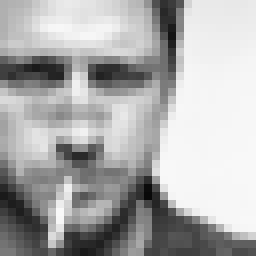
\includegraphics[width=0.3\textwidth]{gerard-butler-noncentered.jpg}
    \caption{a non-ideal sample: the bounding box is offset from the center
             of the face}
    \vfill
    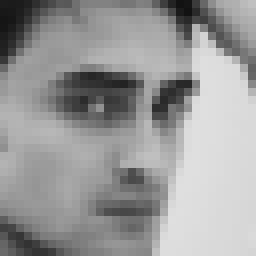
\includegraphics[width=0.3\textwidth]{daniel-radcliffe-angled.jpg}
    \caption{a non-ideal sample: the face is at an angle and the bounding
             box captures the background}
    \end{multicols}
\end{centering}
\end{figure}

However generally the faces can be aligned with one another. The
performance of the classifier could likely be improved by manually
curating a dataset with similar face crops.

Images were collected with \texttt{get\_data.py}.

\subsection{2. Division of processed
images}\label{division-of-processed-images}

120 images of each subject were selected at random from the dataset, and
then were divided randomly into the `training', `validation', and `test'
sets. (data in section 3.), with 100 in `training', and 10 in each
`validation' and `test'

Images were divided randomly with \texttt{create\_samples.py}.

\section{3. K-nearest-neighbors
classification}\label{k-nearest-neighbors-classification}

\subsection{Finding the best value for
k}\label{finding-the-best-value-for-k}

When run on the validation set for values of k in the range
\([1 .. 20]\), the best value for \(k\) was found to be \(k=2\) on the
validation set, with a \(62\)\% accuracy for recognizing an actor from
\(act\).

\subsection{Performance on the test
set}\label{performance-on-the-test-set}

When this value of k was used on the test set, it was correct
\(60.00\)\% of the time. Below are cases where the classifier selected
the wrong face.

\begin{longtable}[c]{@{}llll@{}}
\toprule
input person & input face & nearest person & nearest
neighbor\tabularnewline
\midrule
\endhead
Gerard Butler & 
\includegraphics{assets/person_mismatch/real01.jpg} &
Michael Vartan &
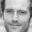
\includegraphics{assets/person_mismatch/recognized01.jpg}\tabularnewline
Daniel Radcliffe & 
\includegraphics{assets/person_mismatch/real02.jpg} &
Michael Vartan &

\includegraphics{assets/person_mismatch/recognized02.jpg}\tabularnewline
Angie Harmon & 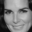
\includegraphics{assets/person_mismatch/real03.jpg} &
Gerard Butler &

\includegraphics{assets/person_mismatch/recognized03.jpg}\tabularnewline
Angie Harmon & 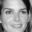
\includegraphics{assets/person_mismatch/real04.jpg} &
Lorraine Bracco &
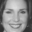
\includegraphics{assets/person_mismatch/recognized04.jpg}\tabularnewline
Peri Gilpin & 
\includegraphics{assets/person_mismatch/real05.jpg} &
Lorraine Bracco &
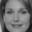
\includegraphics{assets/person_mismatch/recognized05.jpg}\tabularnewline
\bottomrule
\end{longtable}

In general, the mis-recognized nearest neighbors share some attribute
with the input face other than the the person's face, e.g similar
lighting, position of the face in the picture, or framing with bangs.

\section{4. Graph of performance versus
k}\label{graph-of-performance-versus-k}

Accuracy appears to drop off quickly as k increases. This could be
explained if the input dataset were broken into different areas based on
non-face features of the picture (overall light values in the picture,
etc). This would mean that locally knn would perform well, but as k
increased more faces from the same `cluster' would be considered.

\begin{center}
\begin{tikzpicture}[trim axis left, trim axis left]
\begin{axis}[
    xtick=data,
    xlabel=k (samples),
    ylabel=accuracy(percent),
    enlargelimits=0.1,
    ybar interval=0.1,
]
\addplot[scatter, only marks] 
    coordinates {
        (1, 61.67)
        (2, 63.33)
        (3, 58.33)
        (4, 51.67)
        (5, 48.33)
        (6, 50.00)
        (7, 51.67)
        (8, 48.33)
        (9, 50.00)
        (10, 48.33)
        (11, 46.67)
        (12, 46.67)
        (13, 41.67)
        (14, 38.33)
        (15, 38.33)
        (16, 36.67)
        (17, 35.00)
        (18, 35.00)
        (19, 35.00)
        (20, 33.33)
    };
\end{axis}
\end{tikzpicture}
\end{center}

If this were the case, one solution would be to normalize the light
levels in pictures. It could also be solved by clustering faces by their
location in the face-space and performing k-means within each of those
clusters. In general, knn will have these issues though, as without
significant preprocessing, it has no way to distinguish a meaningful
attribute of the input set.

\begin{longtable}[c]{@{}lc@{}}
\toprule
k & person accuracy\tabularnewline
\midrule
\endhead
01 & 61.67\tabularnewline
02 & 63.33\tabularnewline
03 & 58.33\tabularnewline
04 & 51.67\tabularnewline
05 & 48.33\tabularnewline
06 & 50.00\tabularnewline
07 & 51.67\tabularnewline
08 & 48.33\tabularnewline
09 & 50.00\tabularnewline
10 & 48.33\tabularnewline
11 & 46.67\tabularnewline
12 & 46.67\tabularnewline
13 & 41.67\tabularnewline
14 & 38.33\tabularnewline
15 & 38.33\tabularnewline
16 & 36.67\tabularnewline
17 & 35.00\tabularnewline
18 & 35.00\tabularnewline
19 & 35.00\tabularnewline
20 & 33.33\tabularnewline
\bottomrule
\end{longtable}

\clearpage
\newpage

\section{5. Performance of knn classifier on
gender}\label{performance-of-knn-classifier-on-gender}

The best k found for classifying by gender was also \(k=2\), with an
accuracy of \(88.3\)\%.

\begin{center}
\begin{tikzpicture}[trim axis left, trim axis left]
\begin{axis}[
    xtick=data,
    xlabel=k (samples),
    ylabel=accuracy(percent),
    enlargelimits=0.1,
    ybar interval=0.1,
]
\addplot[scatter, only marks] 
    coordinates {
        (1,  86.67)
        (2,  88.33)
        (3,  88.33)
        (4,  85.00)
        (5,  85.00)
        (6,  85.00)
        (7,  88.33)
        (8,  86.67)
        (9,  88.33)
        (10, 85.00)
        (11, 86.67)
        (12, 86.67)
        (13, 81.67)
        (14, 80.00)
        (15, 80.00)
        (16, 76.67)
        (17, 78.33)
        (18, 78.33)
        (19, 75.00)
        (20, 73.33)
    };
\end{axis}
\end{tikzpicture}
\end{center}

\begin{longtable}[c]{@{}lc@{}}
\toprule
k & gender accuracy\tabularnewline
\midrule
\endhead
01 & 86.67\%\tabularnewline
02 & 88.33\%\tabularnewline
03 & 88.33\%\tabularnewline
04 & 85.00\%\tabularnewline
05 & 85.00\%\tabularnewline
06 & 85.00\%\tabularnewline
07 & 88.33\%\tabularnewline
08 & 86.67\%\tabularnewline
09 & 88.33\%\tabularnewline
10 & 85.00\%\tabularnewline
11 & 86.67\%\tabularnewline
12 & 86.67\%\tabularnewline
13 & 81.67\%\tabularnewline
14 & 80.00\%\tabularnewline
15 & 80.00\%\tabularnewline
16 & 76.67\%\tabularnewline
17 & 78.33\%\tabularnewline
18 & 78.33\%\tabularnewline
19 & 75.00\%\tabularnewline
20 & 73.33\%\tabularnewline
\bottomrule
\end{longtable}

This increase in performance is to be expected, since the knn classifier
must be \emph{at least} as good at recognizing a gender as it is at
recognizing an actor / actress from the training set.

\section{6. Performance on gender of actors not in the training
set.}\label{performance-on-gender-of-actors-not-in-the-training-set.}

In order to determine the performance of the classifier on the faces of
people not in the training set, 10 images of Julia Louis-Dreyfus, Dana
Delany, Holly Marie Combs, Cary Elwes, Chris Klein, and Andy Richter
were tested with the gender classifier.

When tested against actors / actresses not in \emph{act}, the knn gender
classifier performs with \(68.3\)\% accuracy. This is notably lower than
the performance on the same actors / actresses in \emph{act}.

It is likely the case that the numbers from part 4 are artificially
inflated - because we are working on the same people as the test set,
the gender classifier can rely on similarities between input images and
the training set that are not necessarily tied to a person's gender.

The actors / actresses used in the test set for this part can be found
in the attached \texttt{different\_actors\_dataset.json}

\end{document}
